%use the KomaScript styling on A4 paper
\documentclass[a4paper]{scrreprt}
%package for citing in Harvard style
\usepackage{natbib}
\bibliographystyle{agsm}
%use UTF-8 encoding
\usepackage[utf8]{inputenc}
\usepackage{graphicx}
\graphicspath{{"./figs"}}

\begin{document}

\begin{titlepage}
\centering
{\large\textsc{Bachelor thesis}\par}
\vspace{8\baselineskip}
{\Huge The right-wing populism of the AfD party and its regional differences\par}
\vspace{2\baselineskip}
{\Large A quantitative analysis on populist antagonisms within the programmatic discourse\par}
\vspace{5\baselineskip}
{\large\textsc{submitted by\\[.5em]Dipl.-Math. Paul Keydel}}
\vfill
{\em Freie Universität Berlin, April 2024}
\end{titlepage}

\tableofcontents

\chapter{Introduction}
The aim of this thesis is to bla bla

\chapter{Populismus im Kontext von Demokratie und Repräsentation}
\section{Ursachen und Typologie des Populismus}
\begin{figure}
    \centering
    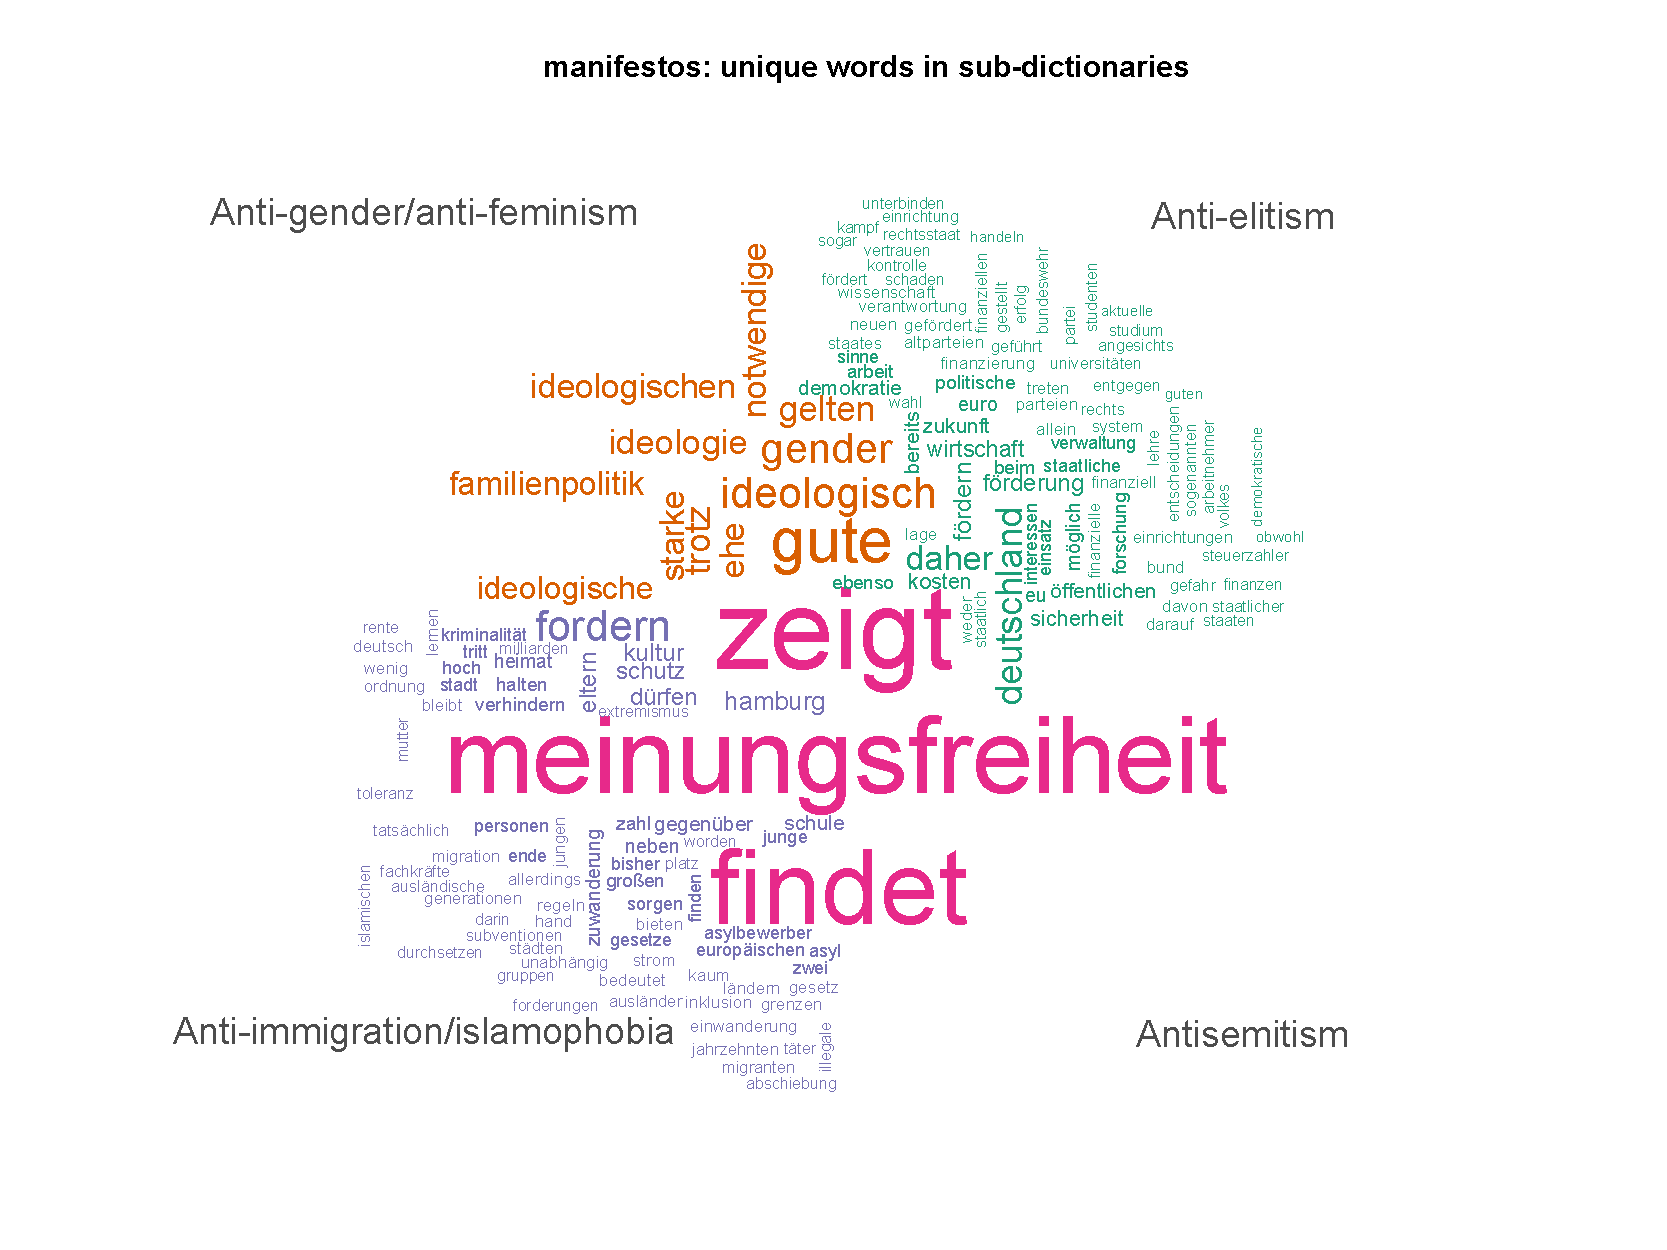
\includegraphics[width=0.9\textwidth]{manifestos_unique_words_subdicts.pdf}
    \caption{a nice plot}
\end{figure}
\begin{figure}
    \centering
    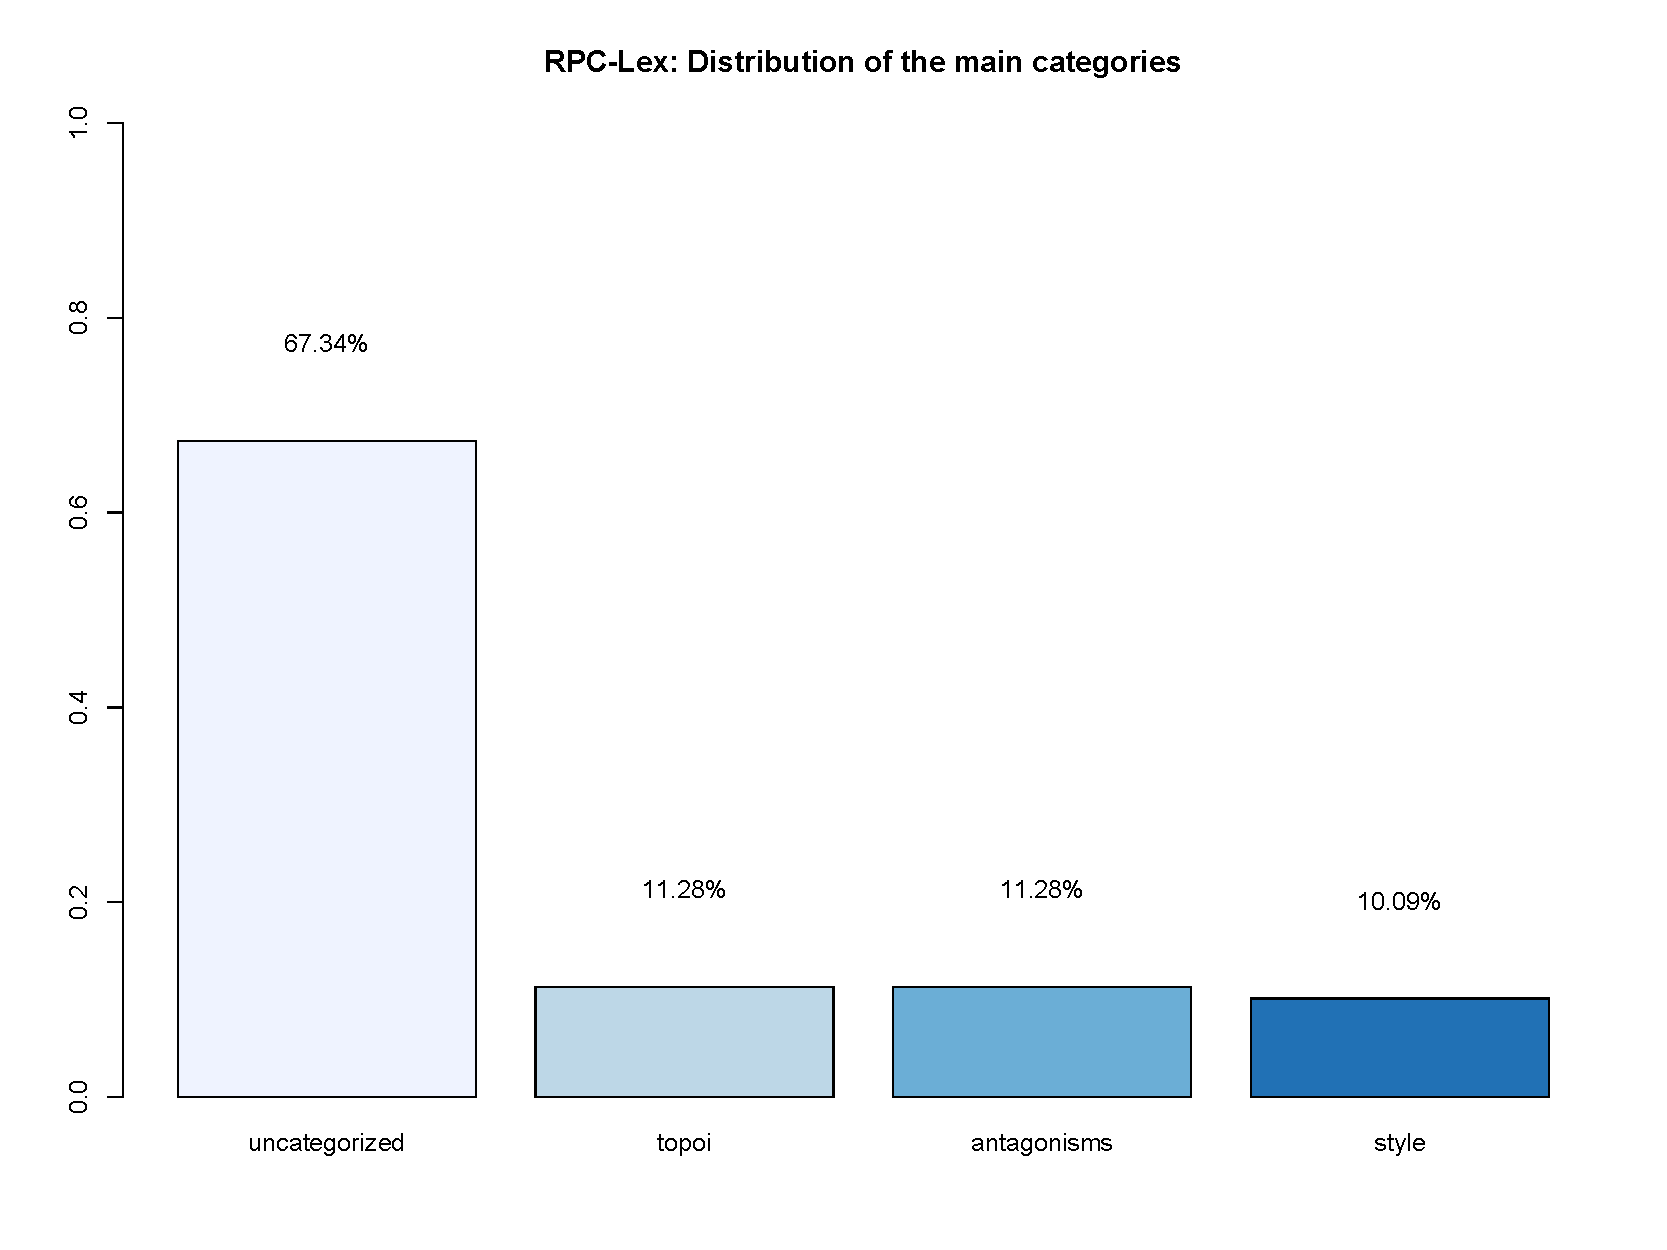
\includegraphics[width=0.9\textwidth]{manifestos_grouped_dict.pdf}
    \caption{a nice plot}
\end{figure}
\begin{figure}
    \centering
    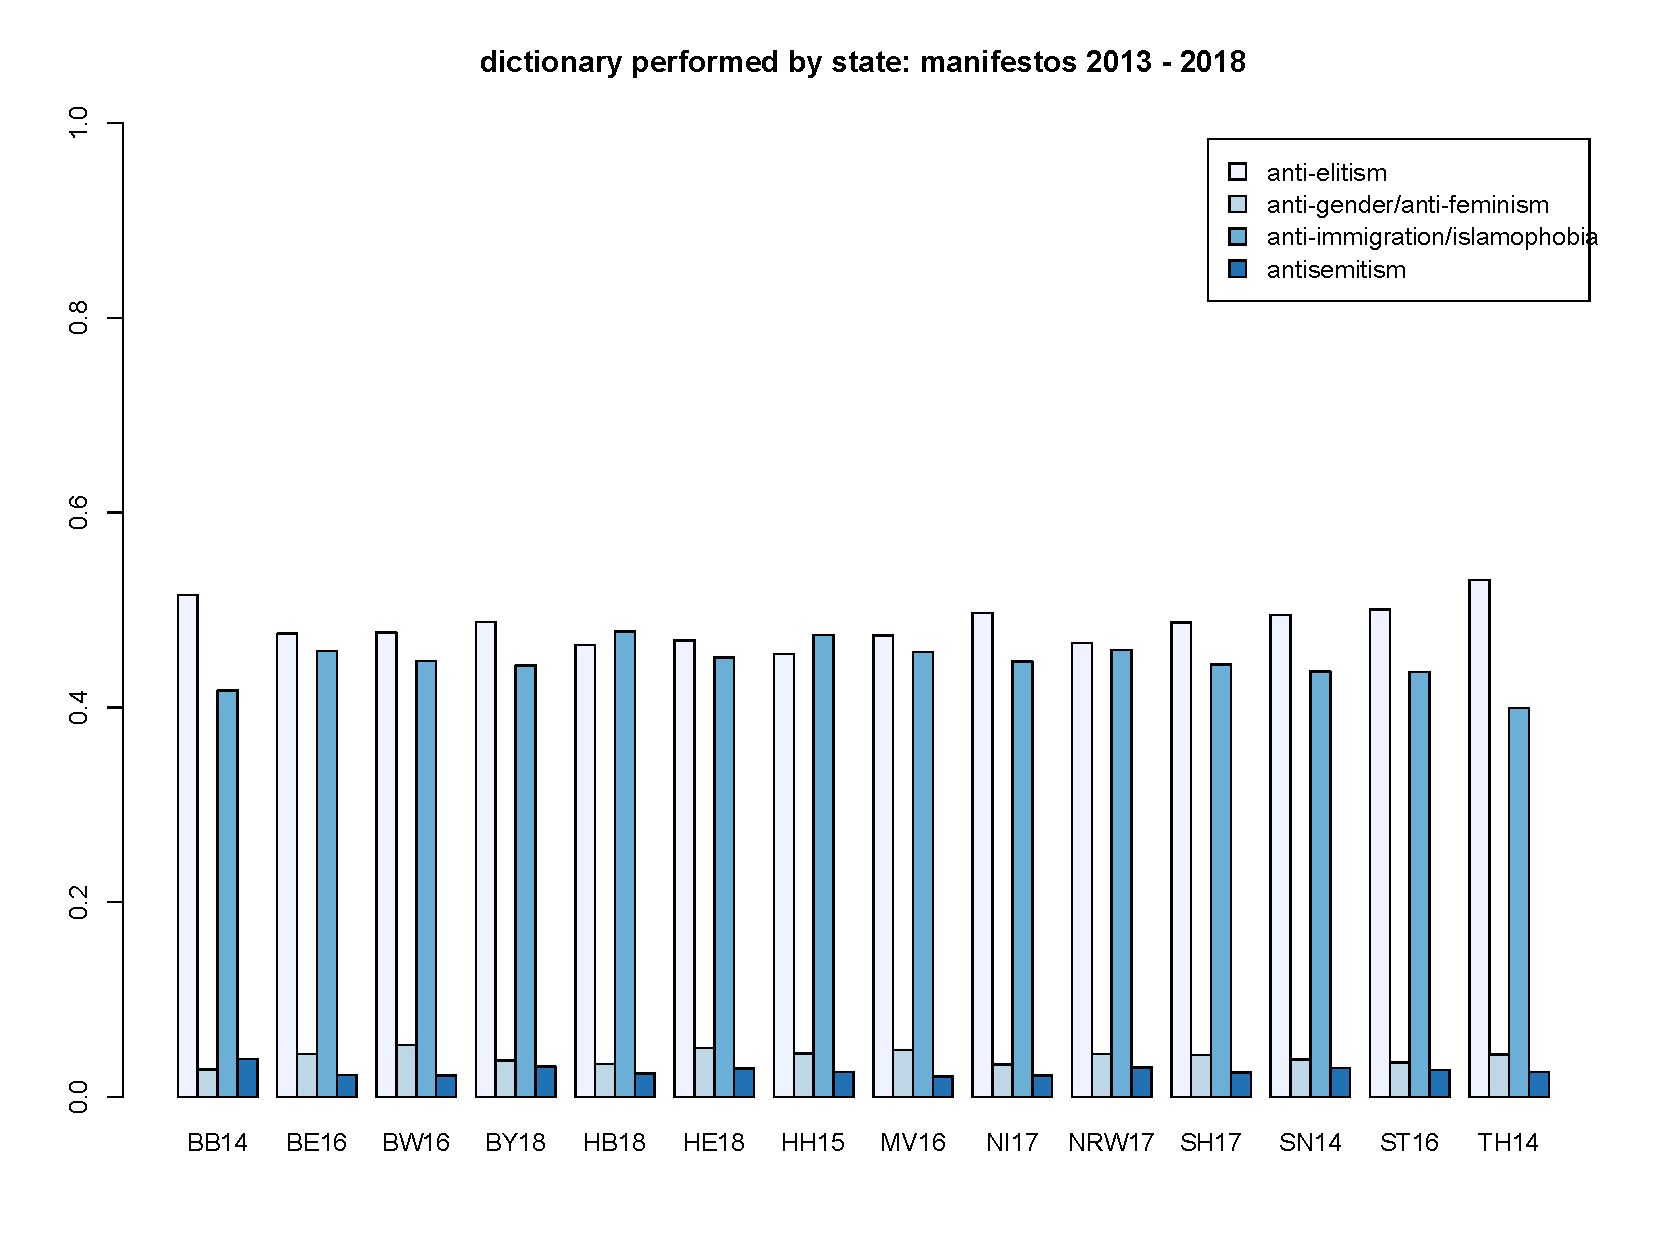
\includegraphics[width=0.9\textwidth]{manifestos_dict_states_2013.pdf}
    \caption{a nice plot}
\end{figure}
\begin{figure}
    \centering
    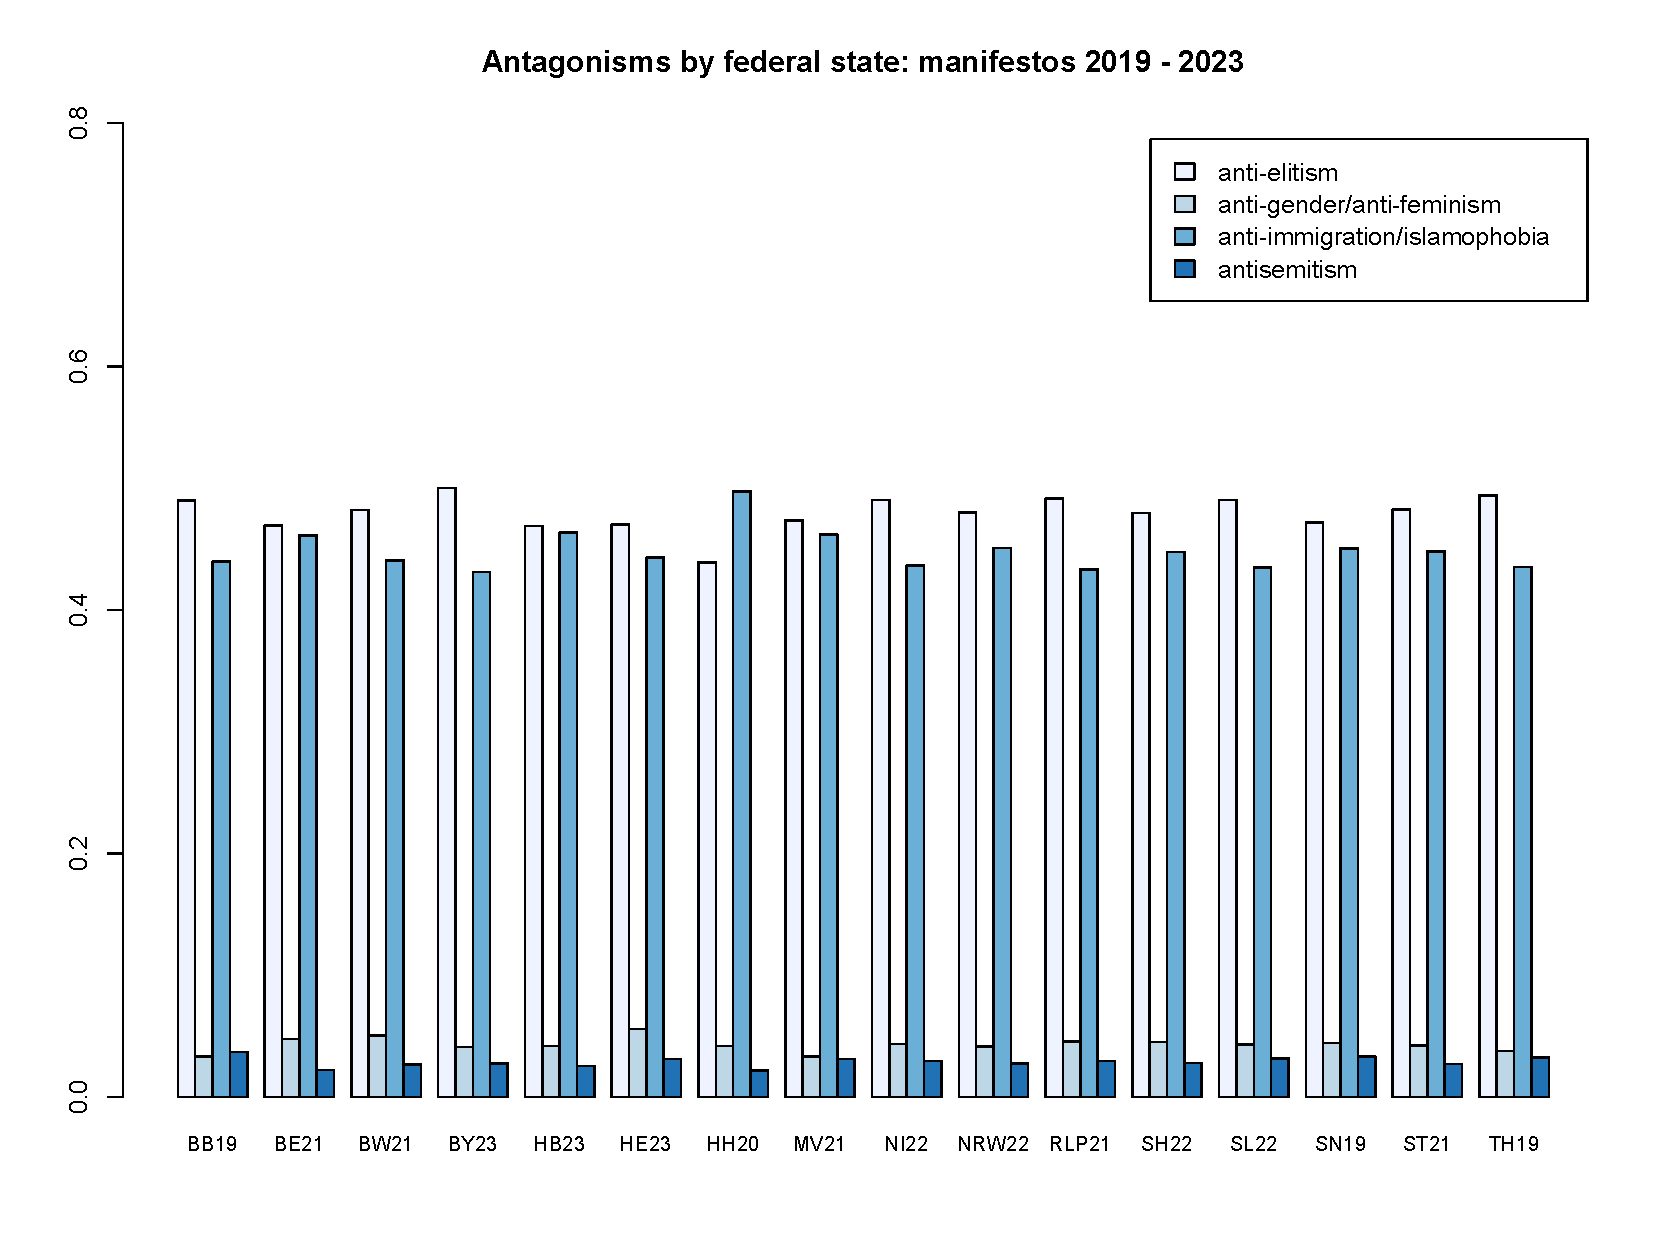
\includegraphics[width=0.9\textwidth]{manifestos_dict_states_2018.pdf}
    \caption{a nice plot}
\end{figure}
\begin{figure}
    \centering
    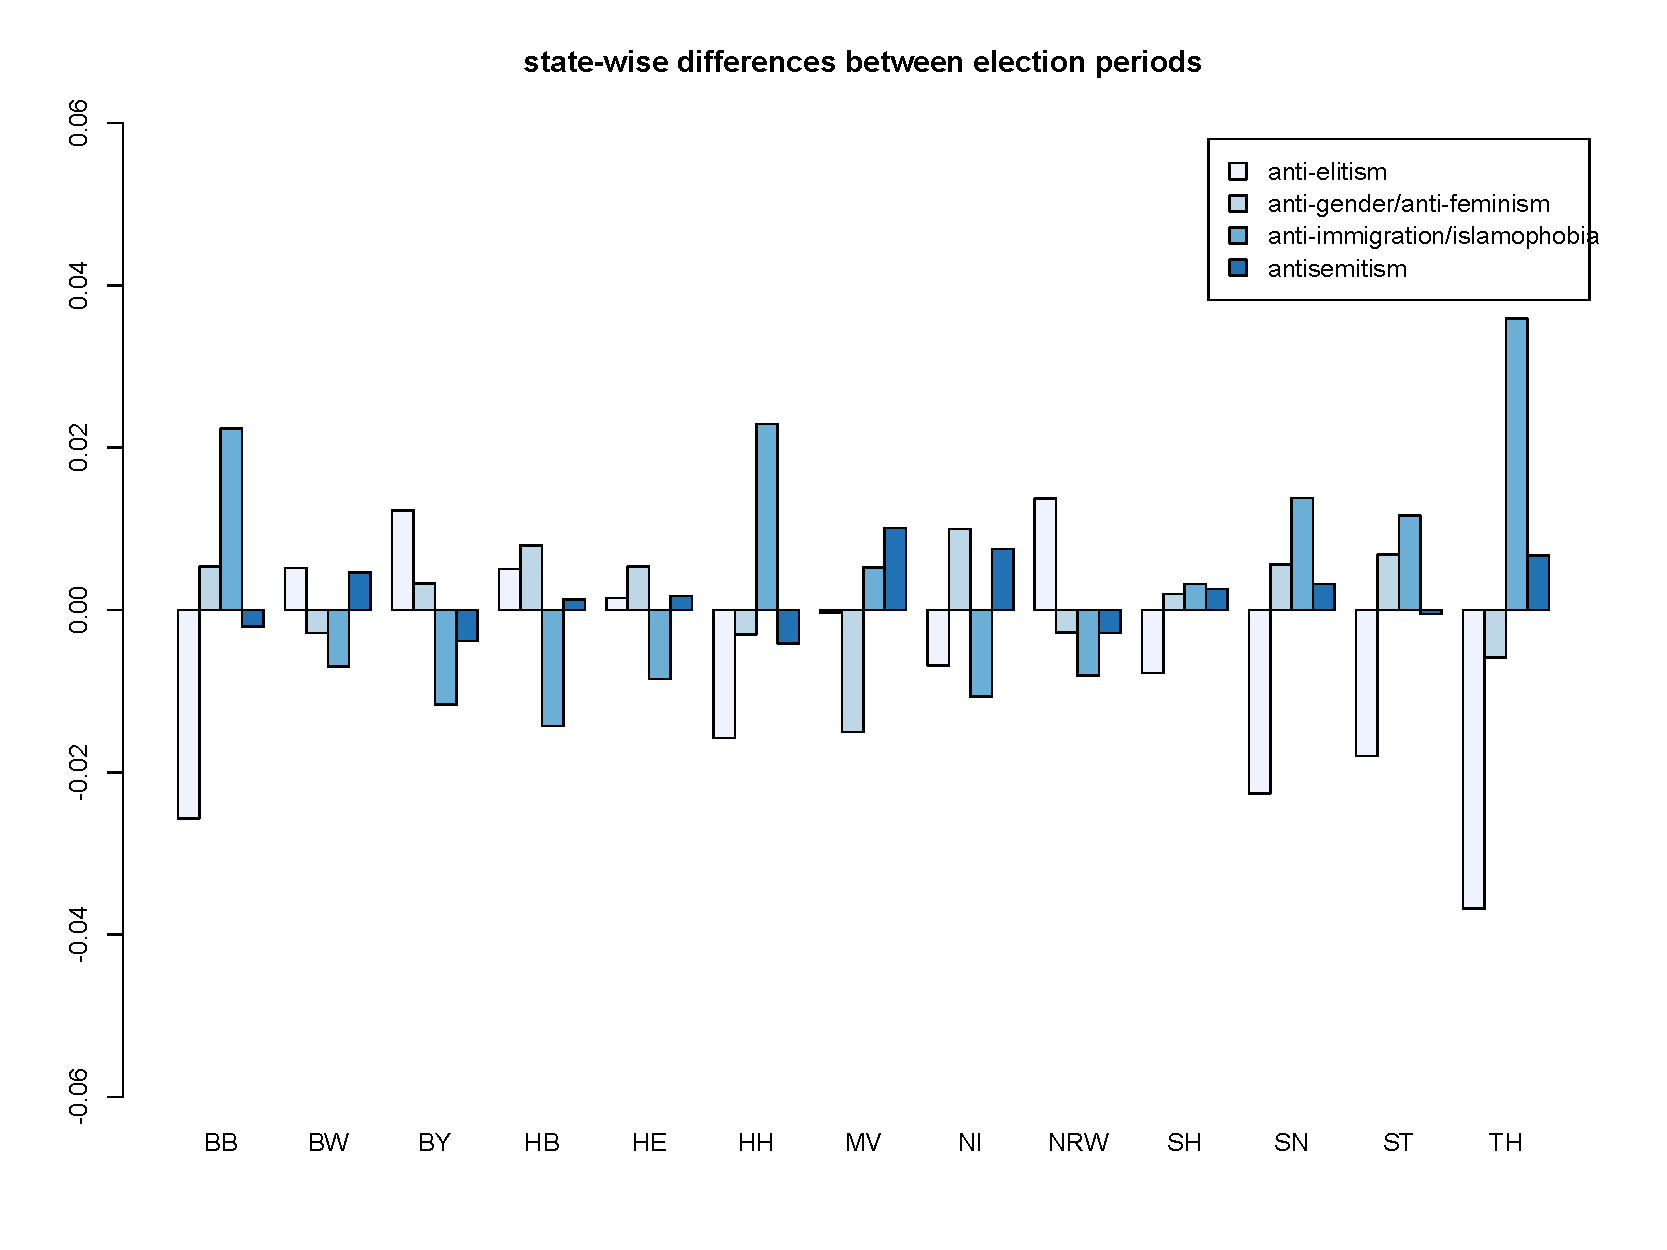
\includegraphics[width=0.9\textwidth]{manifestos_dict_states_diffs.pdf}
    \caption{a nice plot}
\end{figure}
\begin{figure}
    \centering
    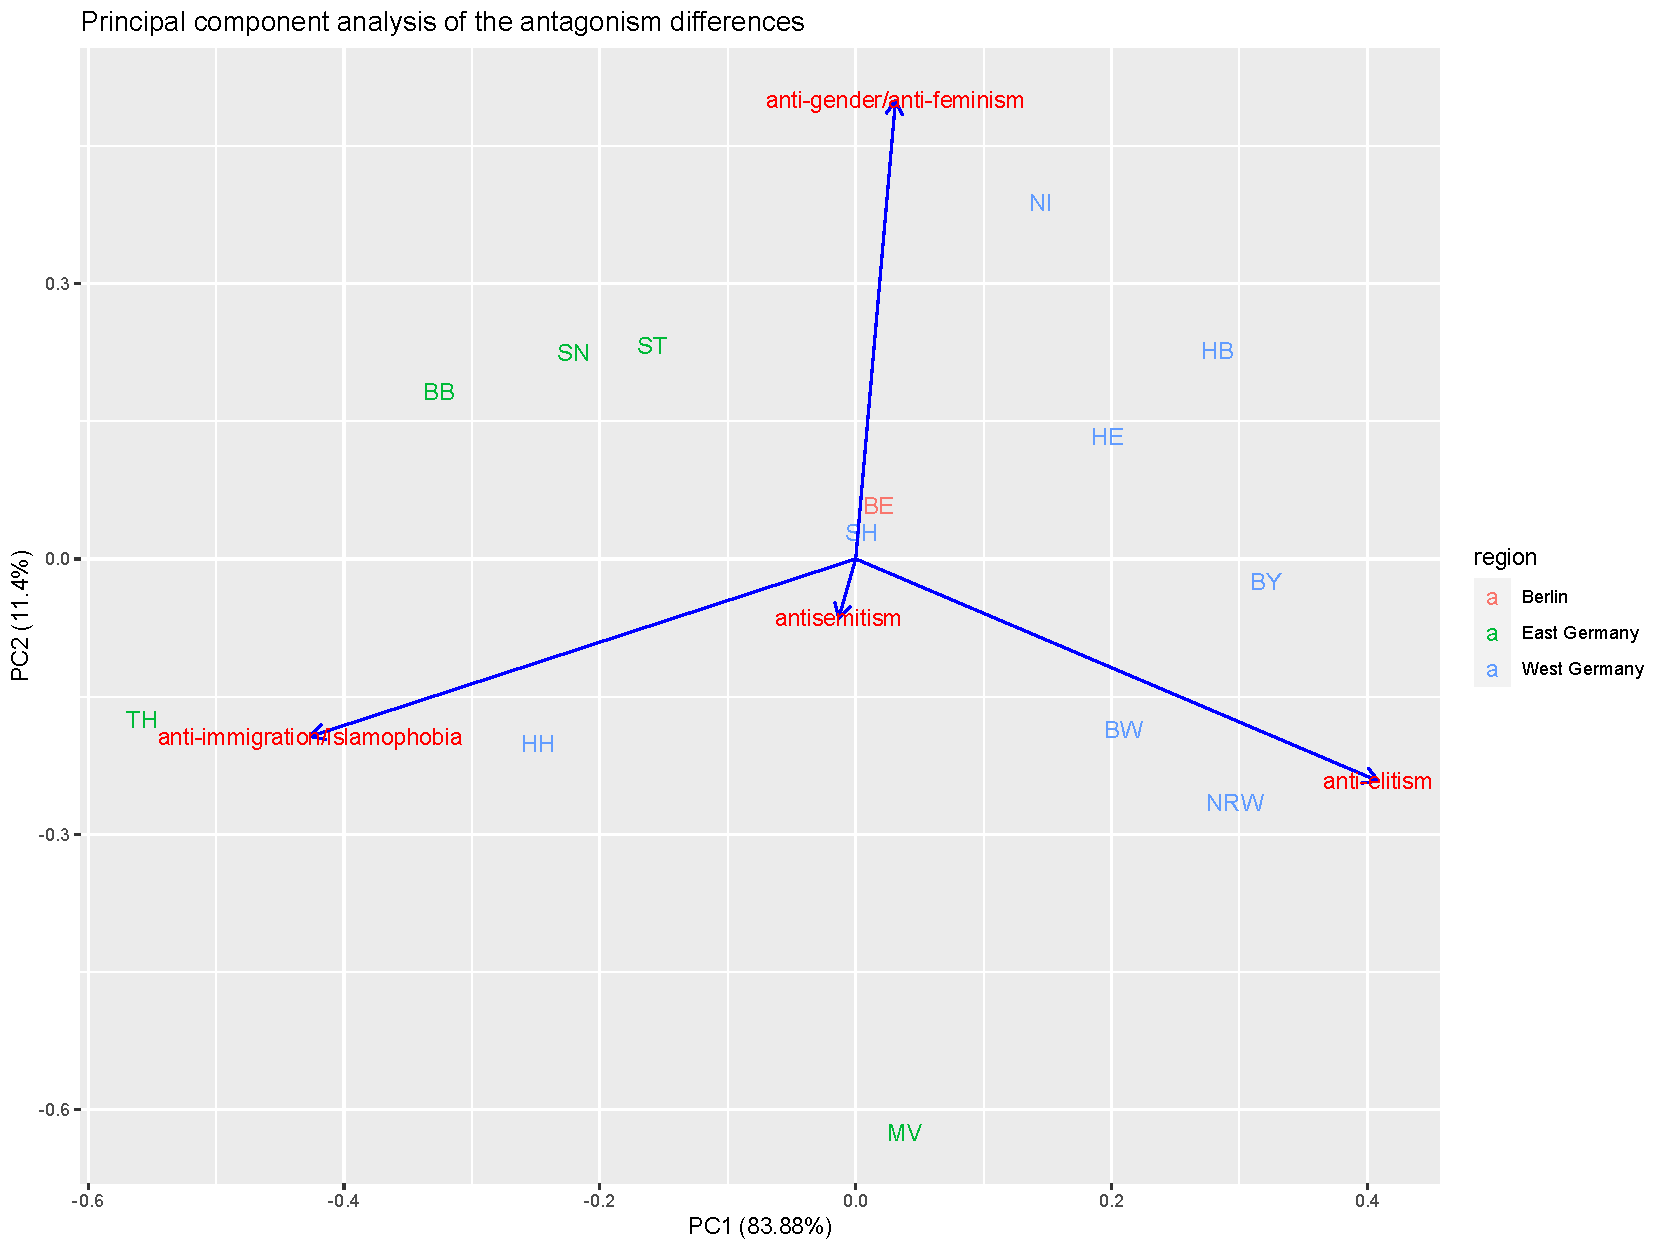
\includegraphics[width=0.9\textwidth]{manifestos_diffs_pca.pdf}
    \caption{a nice plot}
\end{figure}
\begin{figure}
    \centering
    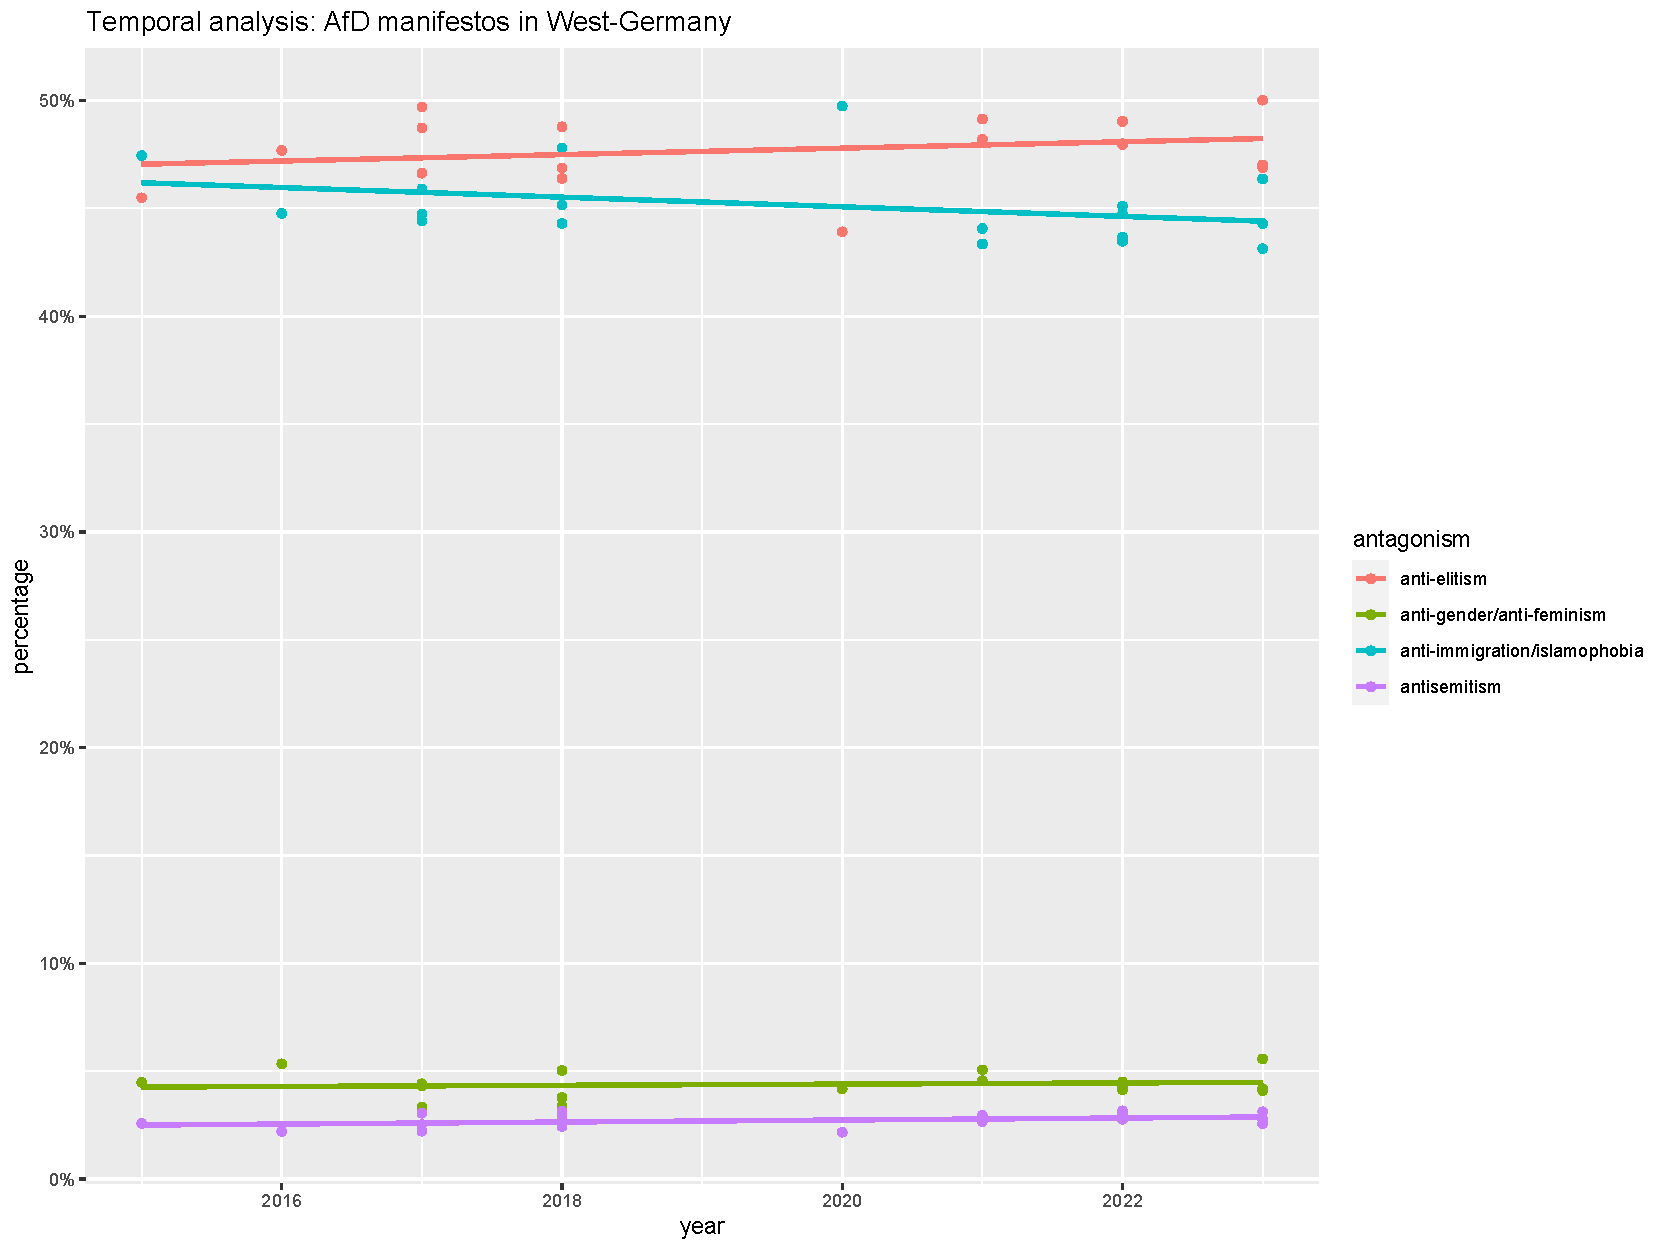
\includegraphics[width=0.9\textwidth]{manifestos_temporal_regression_west.pdf}
    \caption{a nice plot}
\end{figure}
\begin{figure}
    \centering
    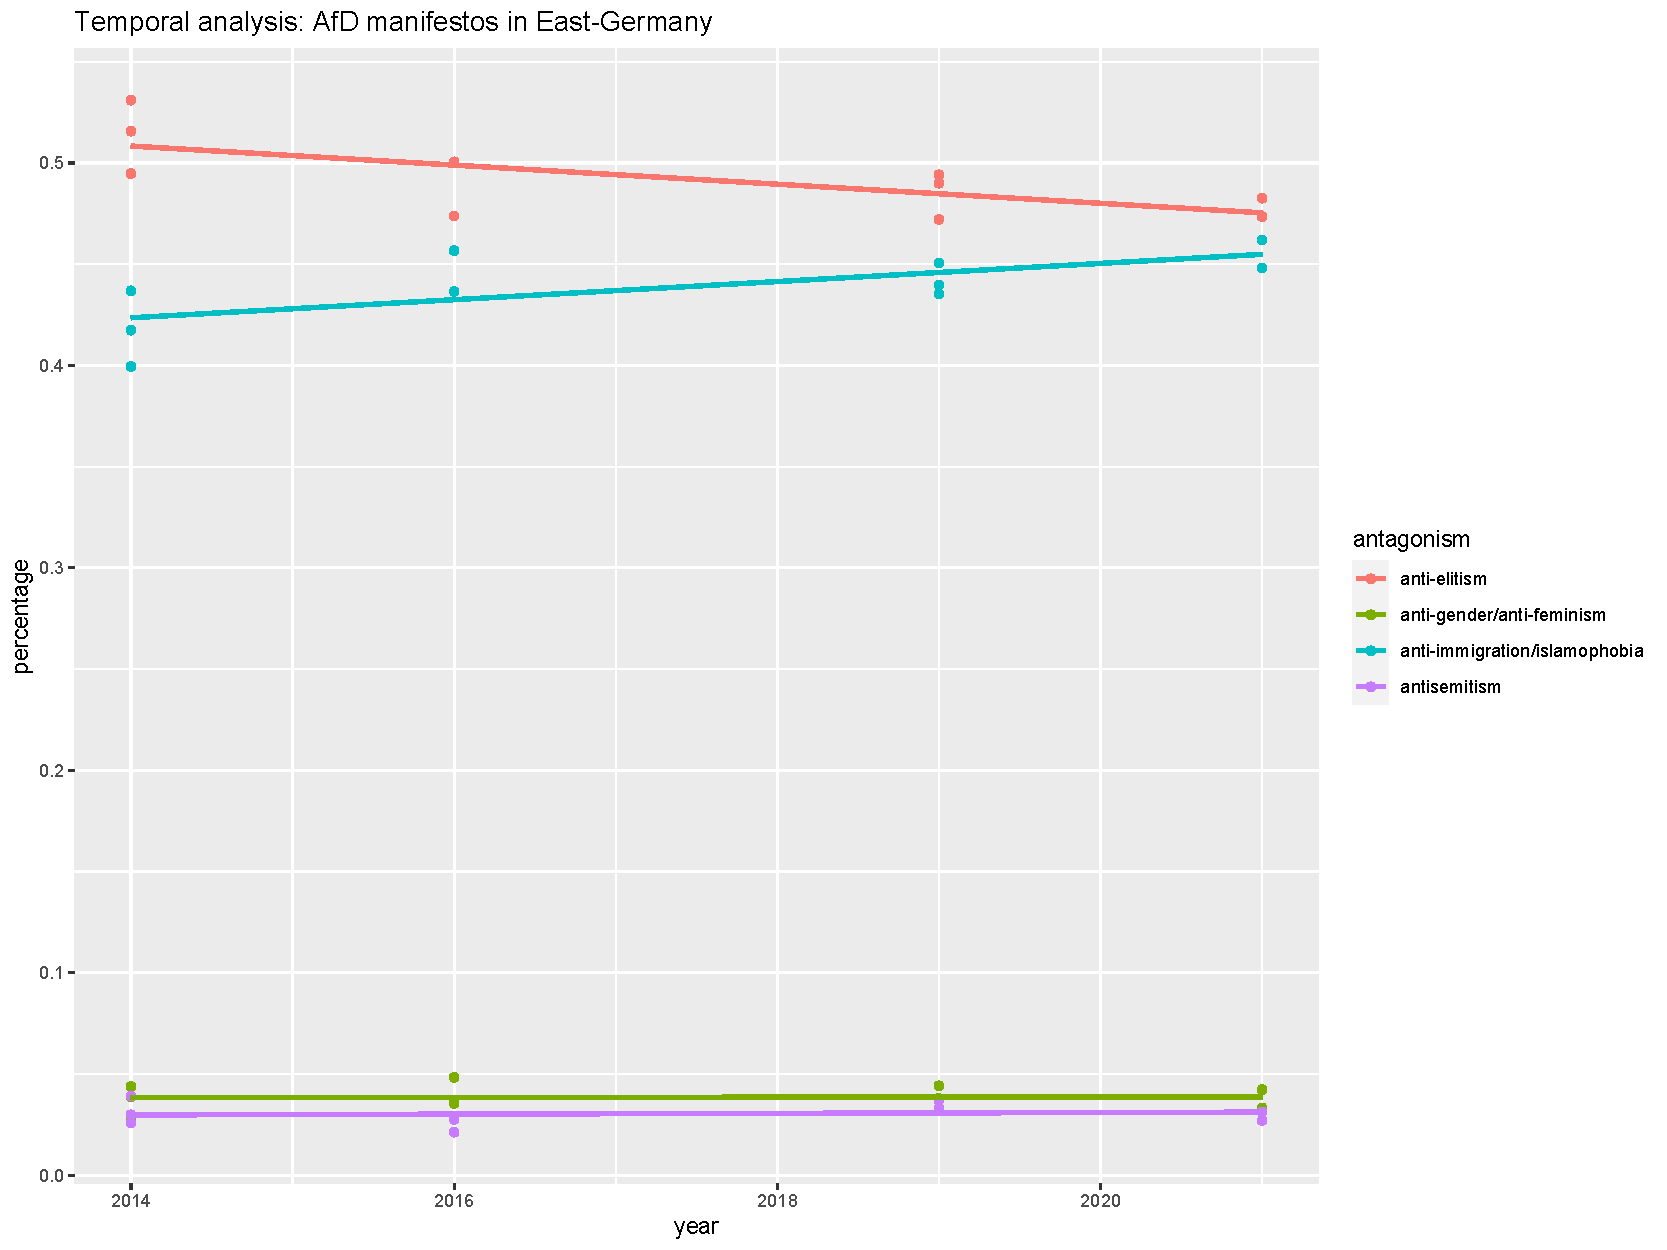
\includegraphics[width=0.9\textwidth]{manifestos_temporal_regression_east.pdf}
    \caption{a nice plot}
\end{figure}
\begin{figure}
    \centering
    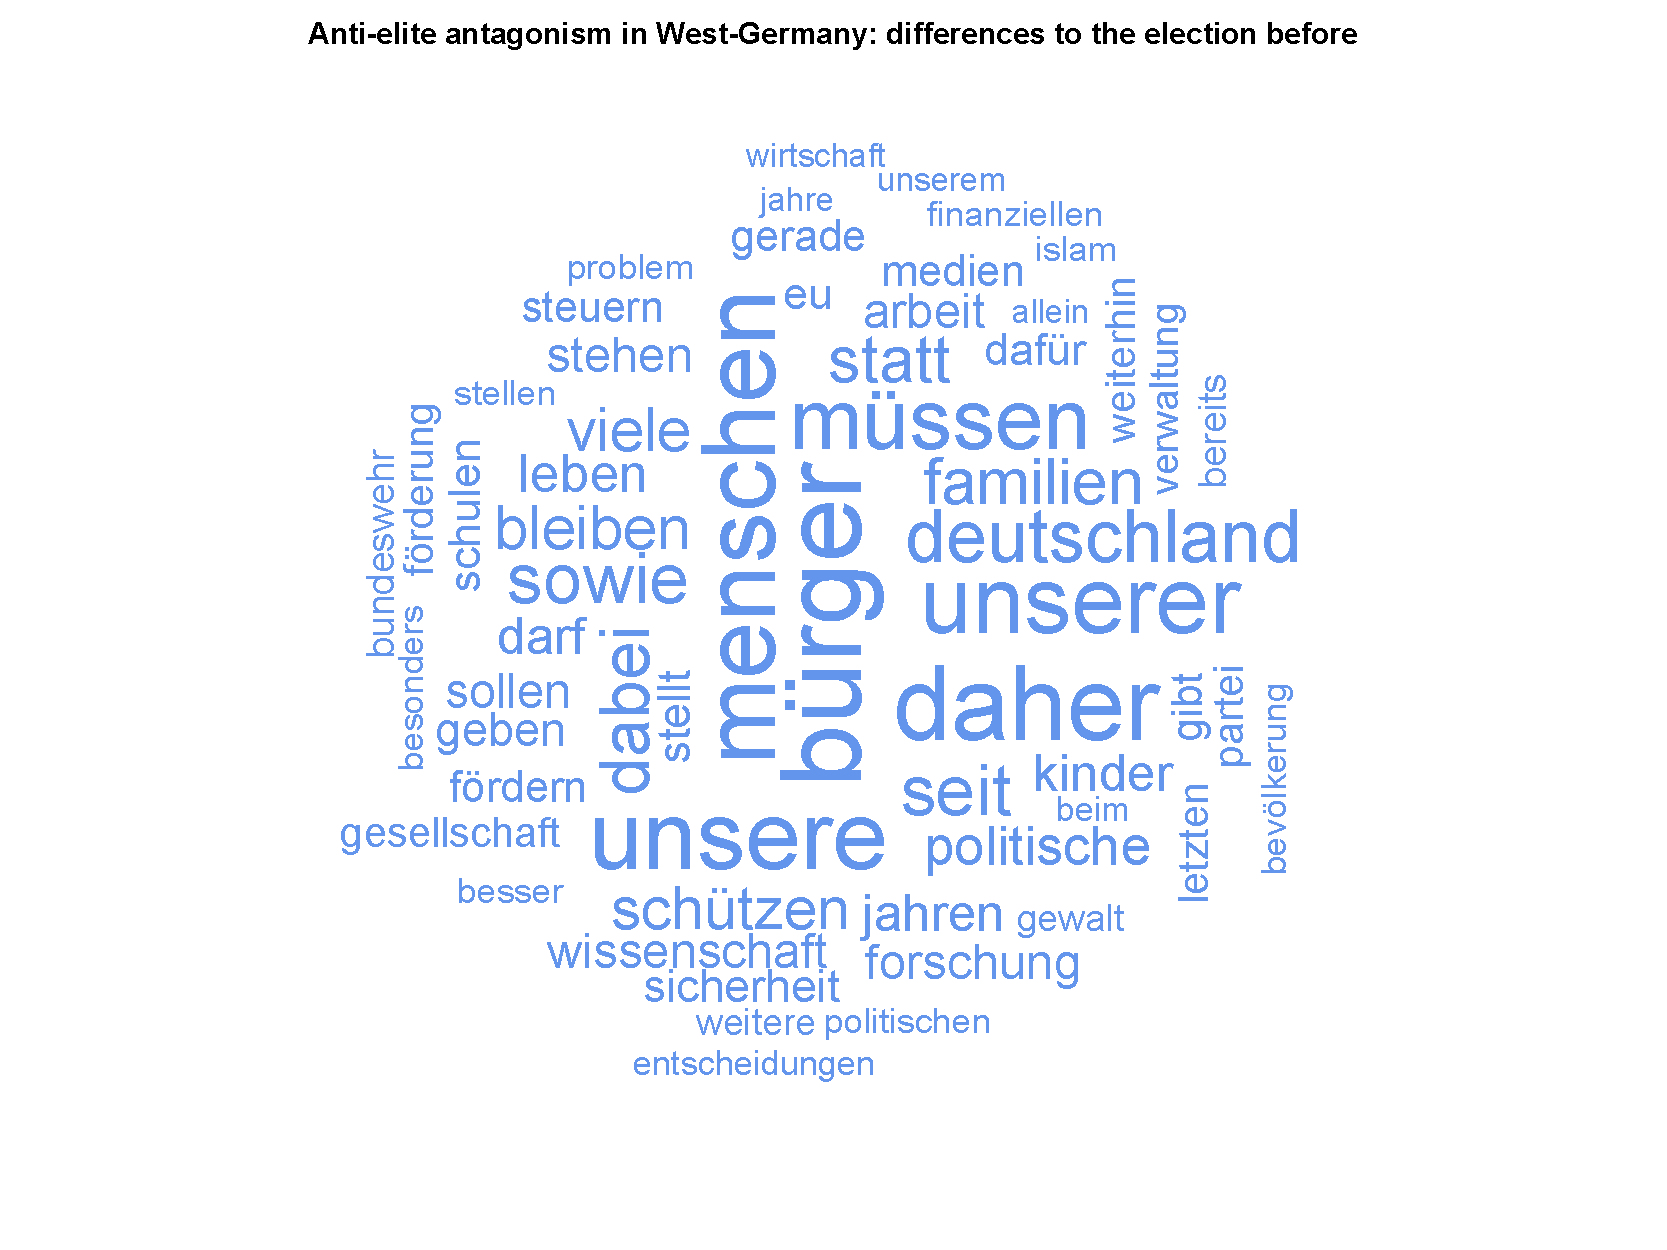
\includegraphics[width=0.9\textwidth]{manifestos_wordcloud_diffs_west.pdf}
    \caption{a nice plot}
\end{figure}
\begin{figure}
    \centering
    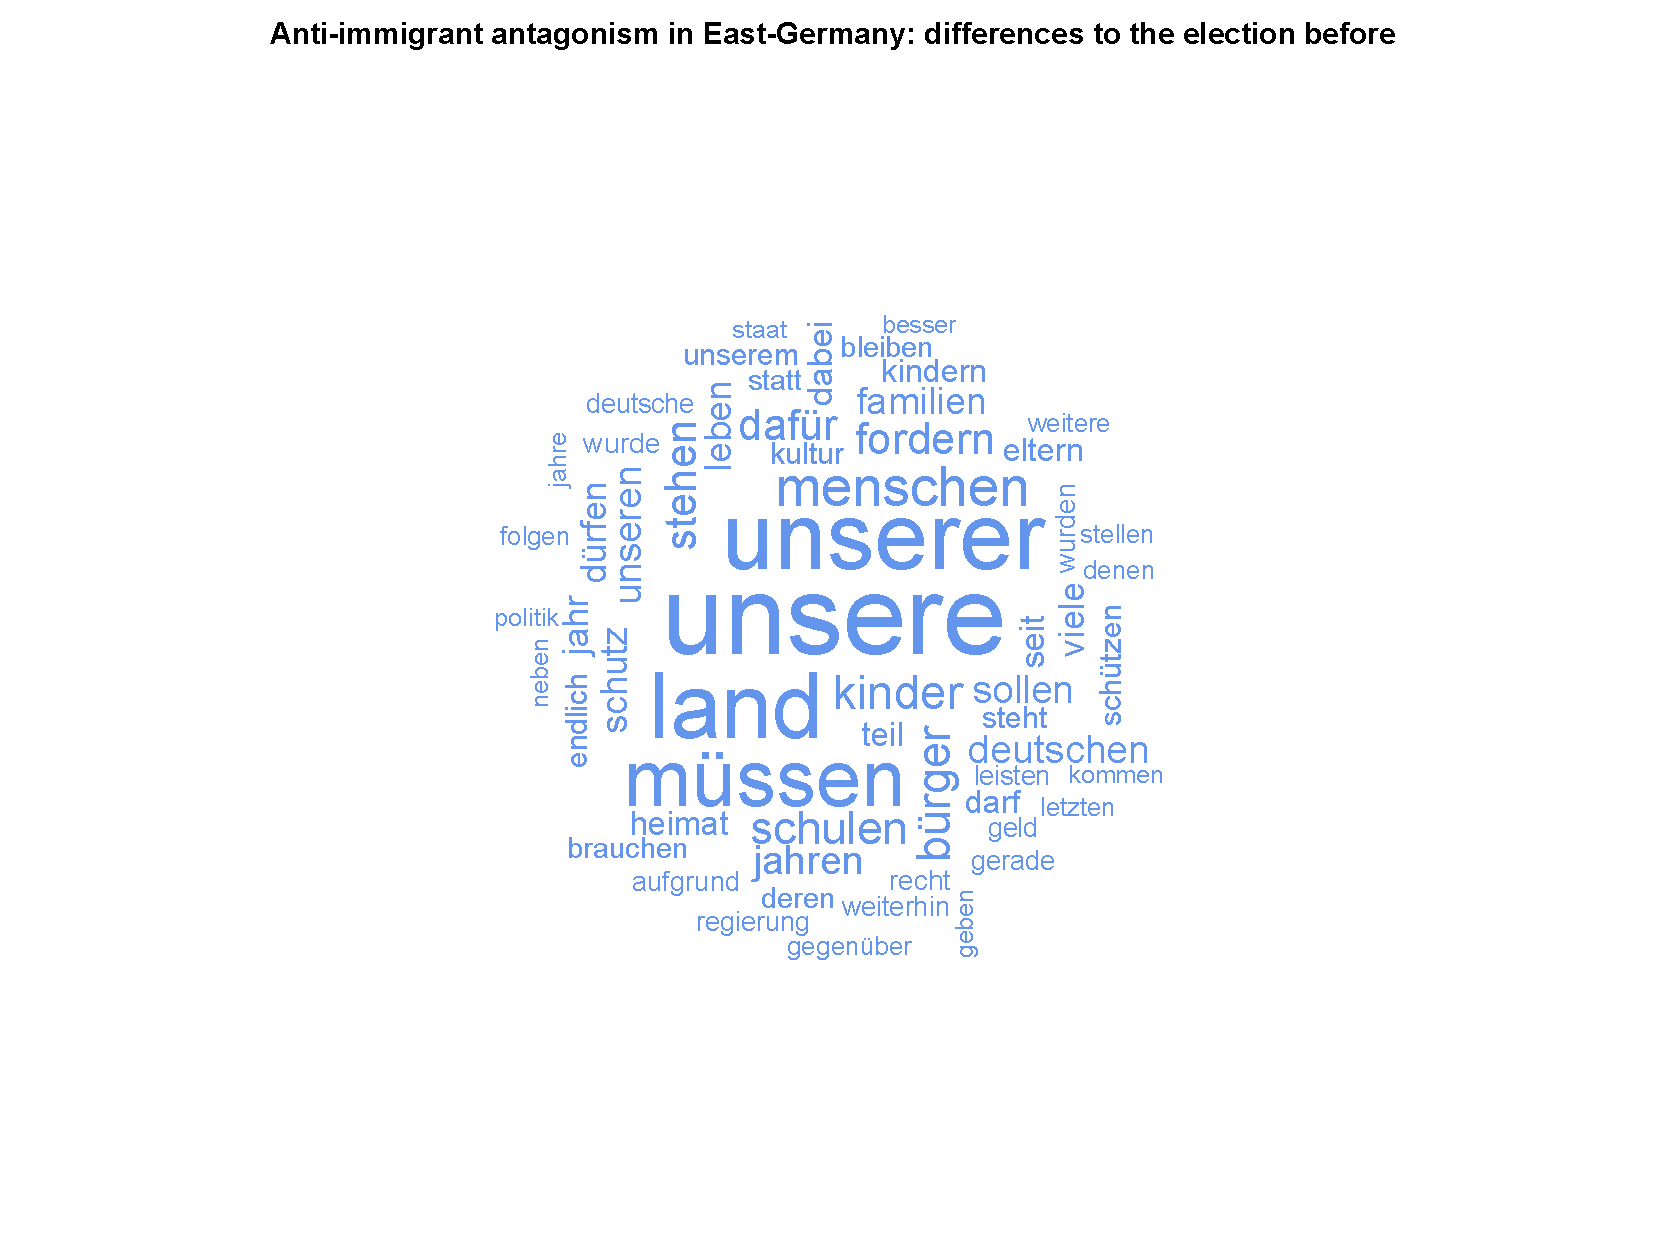
\includegraphics[width=0.9\textwidth]{manifestos_wordcloud_diffs_east.pdf}
    \caption{a nice plot}
\end{figure}

\section{Populismus als Ideologie der Demokratie}
\section{Populismus als Bewegung}
\chapter{Rechtspopulismus und die AfD in Deutschland}
\section{Aktuelle Forschungsdebatte: Rechte Diskurse und die Rolle der AfD}
\section{Unterschiedliche Entwicklungen zwischen Ost und West}
\chapter{Empirische Untersuchungen}
\section{Forschungsdesign}
\section{Entwicklung und Validierung der Dictionaries}
\section{Ergebnisse}
\chapter{Methodenkritik}
\chapter{Fazit und Ausblick}
Let's start citing \citep[p.~22]{canovan:2002}

\bibliography{refs}

\end{document}